%license:BSD-3-Clause
%copyright-holders:Michele Maione
%============================================================
%
%	Piattaforma di cloud gaming per giochi arcade
%
%============================================================

\chapter{Stato dell'arte}
%Nella seconda sezione si riporta lo stato dell’arte del settore, un inquadramento dell’area di ricerca orientato a portare il lettore all’interno della problematica affrontata. Bisogna dimostrare di conoscere le cose fatte fino ad ora in questo campo e il perché si sia reso necessario lo svolgimento di questo lavoro. Questa sezione deve essere grondante di citazioni bibliografiche.
Il capitolo che apre questa tesi fornisce un'introduzione sulla nascita dei videogiochi e dei ricavi globali dell'industria videoludica, dà una definizione di cloud computing e di cloud gaming, fà una panoramica delle piattaforme di gioco che si sono susseguite nel tempo e delle proiezioni di mercato del settore del cloud gaming.




\section{La nascita dei videogiochi}
Nel 1952 nei laboratori dell'Università di Cambridge, come esempio a corredo di una tesi di dottorato sull'interazione uomo-macchina, fu creato OXO, la trasposizione del tris come gioco per computer. OXO è considerato tecnicamente il primo videogioco. Nel 1958 un professore di fisica del Brookhaven National Laboratory creò un gioco, Tennis for Two, che aveva il compito di simulare le leggi fisiche relative ad una partita di tennis, lo strumento utilizzato era un oscilloscopio.

Nel 1961, sei giovani scienziati del Massachusetts Institute of Technology su un PDP-1\footnote{PDP-1: Programmed Data Processor-1, era un computer della Digital Equipment Corporation del 1959.} crearono il primo videogioco a scopo di intrattenimento: Spacewar!.

Due mesi dopo due ingegneri elettrici, N. Bushnell e T. Dabney, terminarono la loro versione di Spacewar! su larga scala (1.500 copie), ma il gioco non ebbe un grande successo a causa dell'elevata difficoltà. Bushnell, dopo l'esperimento non particolarmente riuscito, decise però di insistere nel settore dando così vita alla società Atari. Il primo gioco arcade di Atari fu il primo grande successo del settore: Pong. Pubblicato alla fine del 1972, è un gioco che riproduce approssimativamente la meccanica del ping pong. Atari vendette 19.000 cabinati di Pong e presto molte altre società seguirono l'esempio \parencite{High_Score}. Alla fine del decennio iniziò l'epoca d'oro dei videogiochi arcade e la nascita delle console (console che hanno fatto la storia in Fig. \ref{fig:consoles_history}).

\begin{figure}[H]
	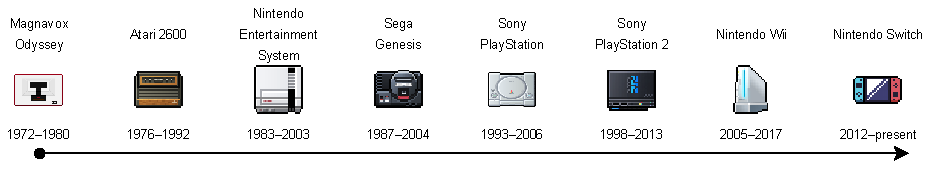
\includegraphics[width=\linewidth]{immagini/consoles_history}
	\caption{Console iconiche, fino alla nona generazione}
	\label{fig:consoles_history}
\end{figure}

I videogiochi sono un mezzo di intrattenimento unico che combina le diverse forme d'arte, quali musica, narrativa e animazione, all'interattività. Ed è proprio questa caratteristica, l'interattività, che permette loro di esercitare un potenziale d'immersione e attrazione che altri media non hanno. Sono ormai diventati un fenomeno culturale di massa con centinaia di milioni di persone che giocano regolarmente ogni giorno, il che li rende attori dominanti nel settore dell'intrattenimento, settore in continua crescita che non ha mai subito interruzioni nel corso degli anni come mostrato in Fig. \ref{fig:valore_commerciale_giochi_globale}. Negli ultimi vent'anni l'importanza economica dei videogiochi arcade è notevolmente diminuita\footnote{Giappone, Cina e Corea mantengono una forte industria arcade ai giorni nostri.} (in viola nella figura) a favore dei videogiochi per personal computer, console e più recentemente per mobile.

\begin{figure}[H]
	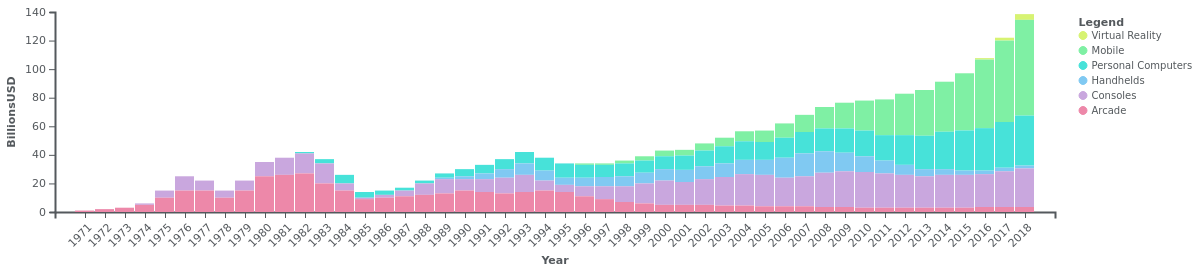
\includegraphics[width=\linewidth]{immagini/valore_commerciale_giochi_globale.png}
	\caption{Ricavi globali dell'industria dei videogiochi dal 1971 al 2018 (non adeguati all'inflazione). Fonte: wikipedia.org}
	\label{fig:valore_commerciale_giochi_globale}
\end{figure}



\section{Cloud gaming}
Negli ultimi anni sono apparsi molti tipi di servizi che sfruttano il paradigma del cloud computing: archiviazione (Dropbox, Drive, OneDrive), musica (Spotify, Amazon Music), cinematografia (Prime Video, Netflix), documenti (Google Workspace, Office 365) e più recentemente il cloud gaming. Il cloud gaming è un servizio che unisce il cloud computing e il live streaming per rendere possibile giocare in remoto senza scaricare o installare il gioco sul device dell'utente, in pratica consente di archiviare ed eseguire i videogiochi su un server remoto e trasmettere l'output audio-video all'utente sul proprio dispositivo.

Il cloud computing è un paradigma in cui un provider offre risorse fisiche e software accessibili da remoto, tramite la sottoscrizione di un abbonamento mensile/annuale oppure "pay-as-you go" (calcolato su: spazio di archiviazione utilizzato, tempo di utilizzo, cicli di CPU/GPU, ecc\dots), le cui caratteristiche essenziali sono:

\begin{itemize}
	\item La capacità di fornire risorse hardware (processori, memoria, spazio di archiviazione, ecc\dots) automaticamente in base alle necessità software;
	\item L'accesso alle risorse attraverso la rete tramite protocolli standard;
	\item Le risorse fisiche e virtuali possono essere distribuite dinamicamente agli utenti in base alle loro richieste;
	\item Dal punto di vista dell'utente le risorse sono illimitate e possono essere acquistate in qualsiasi quantità ed in qualunque momento.
	\item L'uso delle risorse e dei servizi è ottimizzato tramite il modello "pay-per-use" ed è monitorato e controllato in modo trasparente sia dal provider che dall'utente; alcune società offrono anche abbonamenti mensili e annuali, che invece limitano le risorse ad un tetto massimo.
\end{itemize}

Il cloud computing offre tre modelli di servizio: \emph{Infrastructure as a Service} (IaaS), \emph{Platform as a Service} (PaaS) e \emph{Software as a Service} (SaaS). Il cloud gaming è l'unione del modello SaaS poichè i videogiochi sono offerti come un servizio dal punto di vista del giocatore, e del modello PaaS dal punto di vista dello sviluppatore che necessita del sistema operativo, delle librerie e dei kit di sviluppo; per cui il paradigma implementato dal cloud gaming è definito \emph{Gaming as a Service} (GaaS) e si divide in tre instanze \parencite{Cloud_for_Gaming}, come mostrato in Fig. \ref{fig:GaaS}, che sono:

\begin{itemize}
	\item \emph{Remote rendering} (RR-GaaS): il gioco viene eseguito e codificato sul server ed inviato all'utente come un filmato;
	\item \emph{Local rendering} (LR-GaaS): il gioco viene eseguito, codificato sul server ed inviato all'utente sotto forma di istruzioni di rendering. Il client invia le istruzioni di rendering alla scheda grafica dell'utente;
	\item \emph{Cognitive resource allocation} (CRA-GaaS): il client riceve moduli eseguibili del gioco che vengono eseguiti sul dispositivo dell'utente.
\end{itemize}

\begin{figure}[H]
	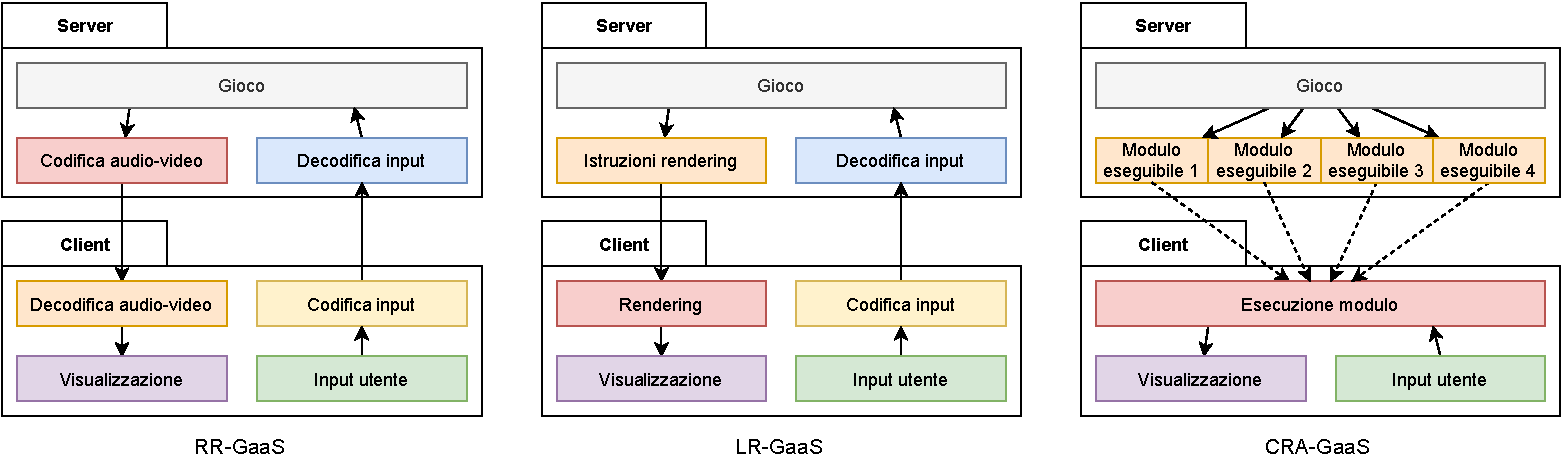
\includegraphics[width=\linewidth]{immagini/GaaS}
	\caption{Instanze di GaaS}
	\label{fig:GaaS}
\end{figure}

Il rendering remoto (RR-GaaS) è attualmente l'istanza più utilizzata nelle soluzioni di cloud gaming sul mercato essendo la soluzione che ha tutta la computazione a carico del server ed offre all'utente la possibilità di usare videogiochi computazionalmente esosi su qualsiasi tipo di device. Dei tre protocolli è però quello che richiede il bit-rate maggiore. Alcuni esempi sono Stadia\footnote{Stadia è una piattaforma di cloud gaming di Google.}, PlayStation Now\footnote{PlayStation Now è il cloud gaming targato Sony.}.

Il rendering locale (LR-GaaS) è l'istanza che richiede il bit-rate minore ma, come nel caso dell'allocazione delle risorse, il rendering è eseguito sul device dell'utente, richiedendo così particolari caratteristiche hardware. Attualmente non ci sono importanti piattaforme sul mercato che offrono questo tipo d'istanza.

Alcune società propongono una versione dell'allocazione delle risorse cognitive (CRA-GaaS) mista al rendering remoto, in cui il gioco viene inizialmente servito come rendering remoto ed in contemporanea viene eseguito il download dei moduli eseguibili; al completamento del download dei moduli che riguardano l'attuale stato del gioco, lo streaming si interrompe e il gioco riprende dal device dell'utente; questa è una delle funzionalità che Project Atlas\footnote{Project Atlas è un progetto di una piattaforma cloud gaming mista ad intelligenza artificiale della Electronic Arts.} dovrebbe offrire. Un'altra variante, che viene chiamata commercialmente come "progressive download", si basa sul concetto di scaricare inizialmente i moduli principali del gioco, solitamente il menù e il primo livello; gli store Origin\footnote{Origin è una piattaforma di distribuzione digitale di videogiochi sviluppata da Electronic Arts.} e Ubisoft Connect\footnote{Ubisoft Connect è un servizio di distribuzione digitale della società Ubisoft.} implementano questa funzionalità.

Nel prossimo paragrafo vedremo le tecnologie per lo streaming maggiormente usati.



\subsection{Tecnologie per lo streaming audio-video}
I protocolli di comunicazione a livello di trasporto su cui sono costruiti servizi, tecnologie e Web API \parencite{Audio_and_video_delivery}, schematizzati in Fig. \ref{fig:webprotocols}, sono UDP, TCP e SCTP, le cui caratteristiche principali sono riassunte in Tabella \ref{table:TransportLayerComp}.

\begin{table}[H]
	\centering
	\begin{tabular}{||l c c c||} 
		\hline
		Caratteristica & UDP & TCP & SCTP \\
		\hline\hline
		Dimensione header & 8 byte & 20-60 byte & 12 byte \\
		\hline
		Entità del pacchetto & datagramma & segmento & datagramma \\
		\hline
		Orientato alla connessione & no & sì & sì \\
		\hline
		Trasporto affidabile & no & sì & sì \\
		\hline
		Consegna ordinata & no & sì & sì/no \\
		\hline
		Controllo del flusso & no & sì & sì \\
		\hline
		Controllo della congestione & no & sì & sì \\
		\hline
		Flussi multipli & no & no & sì \\
		\hline
		Multihoming\tablefootnote{Il multihoming è la funzionalità di poter connettere un host a più di una rete.} & no & no & sì \\
		\hline
	\end{tabular}

	\caption{Comparazione tra protocolli di trasporto}
	\label{table:TransportLayerComp}
\end{table}

Di questi solo quattro possono essere utilizzati per lo streaming utilizzando il browser web \parencite{High_Performance_Browser_Networking}:

\begin{itemize}	
	\item Dynamic Adaptive Streaming over HTTP (DASH) è una tecnica di streaming con bit-rate adattivo del Moving Picture Experts Group (MPEG), che consente lo streaming di alta qualità di contenuti multimediali su protocollo HTTP;
	\item HTTP Live Streaming (HLS) è il protocollo di streaming ad alta latenza più popolare su HTTP per video on demand (video preregistrato) sviluppato da Apple;
	\item WebSocket è un protocollo di comunicazione che fornisce un canale full-duplex su una singola connessione TCP, con una latenza inferiore rispetto ad HLS e DASH;
	\item Web Real-Time Communication (WebRTC) è un progetto per la comunicazione in tempo reale basato sul protocollo RTP (Real-time Transport Protocol).
\end{itemize}

\begin{figure}[H]
	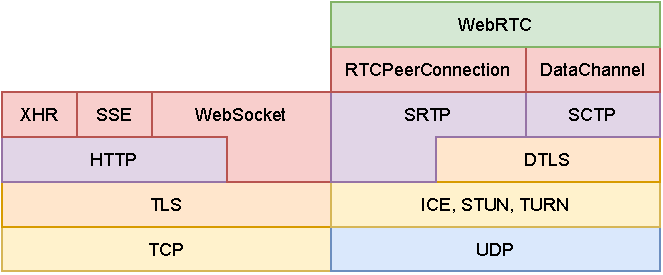
\includegraphics[width=\linewidth]{immagini/webprotocols}
	\caption{Streaming con perdita di pacchetti dell'8\%.}
	\label{fig:webprotocols}
\end{figure}

Nel paradigma del cloud gaming la codifica audio-video avviene in real-time e il buffering non è usabile perché aumenterebbe la latenza, per questi motivi non tutte le tecnologie citate sono adatte. Come vedremo nelle caratteristiche delle piattaforme di streaming commerciali, descritte nel prossimo paragrafo, solo TCP, UDP ed RTP sono stati effettivamente usati. Solitamente la comunicazione tramite TCP è relegata alla parte di autenticazione e gestione dell'input utente. Infatti da test condotti in \parencite{Network_technology_for_transmission_of_visual_information} sul frame rate in caso di perdita di pacchetti durante lo streaming, in Fig. \ref{fig:fps_in_protocols} con una perdita di pacchetti dell'8\%, si nota che con RTSP\footnote{RTSP: Real Time Streaming Protocol serve a stabilire e gestire la sessione di streaming, la trasmissione dei dati avviene tramite RTP e la raccolta delle statistiche sulla qualità del servizio è affidata al Real-time Transport Control Protocol (RTCP).}, schema (a) e (b), il frame rate è costante ma con alcune perturbazioni; invece HLS, schema (c), risulta essere la tecnologia che risente maggiormente della perdita dei pacchetti; mentre con RTMP\footnote{RTMP: Real Time Messaging Protocol era un protocollo sviluppato da Macromedia per il Flash player, ad oggi non più supportato dai browser.}, schema (d), la riproduzione si interrompe e il video si blocca per alcuni secondi.

\begin{figure}[H]
	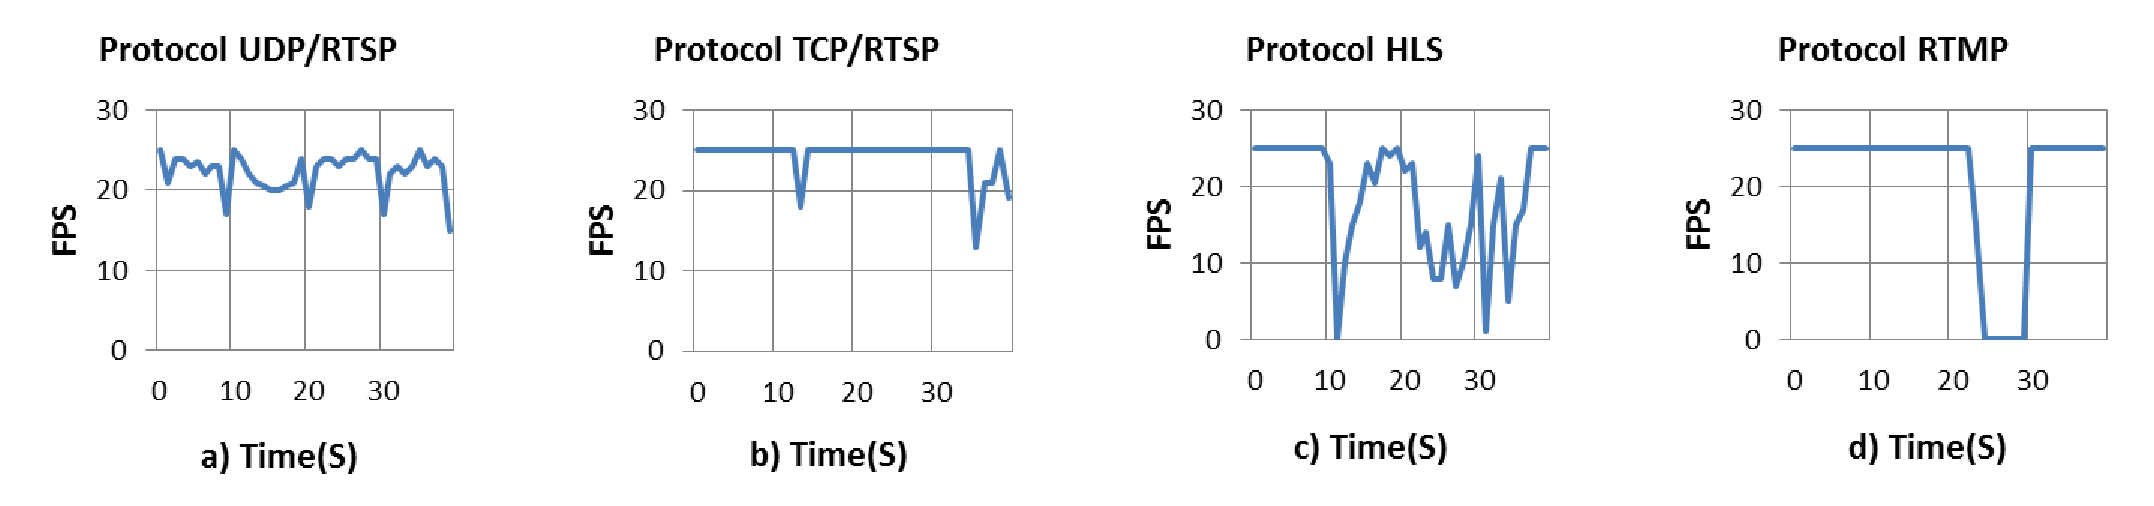
\includegraphics[width=\linewidth]{immagini/fps_in_protocols}
	\caption{API, protocolli e servizi di rete del browser}
	\label{fig:fps_in_protocols}
\end{figure}

Nel prossimo paragrafo viene fatta un'introduzione, in ordine cronologico, delle piattaforme di cloud gaming sul mercato.

\subsection{Storia del cloud gaming} \label{StoriaDelCloudGaming}
Una delle prime piattaforme di cloud gaming è stata OnLive di OL2, presentata alla GDC\footnote{GDC: Game Developers Conference, una conferenza annuale per gli sviluppatori di videogiochi.} 2009 e poi lanciata sul mercato a giugno 2010 negli Stati Uniti e a settembre 2011 nel Regno Unito. I giocatori, previo pagamento di un abbonamento mensile di 15\$, potevano acquistare o noleggiare giochi sulla piattaforma oppure utilizzare quelli precedentemente acquistati su Steam\footnote{Steam è un servizio di distribuzione digitale di videogiochi della società Valve.}. Il servizio era ospitato su 5 data center situati sul suolo americano che servivano gli utenti per vicinanza geografica; il bit-rate richiesto era di 1,5 Mbps per la qualità video SD\footnote{SD: Standard Definition include i formati video con rapporto 4:3 e 16:9 con 480 linee di risoluzione (in alcuni casi 576).} e 5 Mbps per la Standard HD\footnote{Standard High Definition (chiamata anche HD ready) è un formato video 16:9 (disponibile anche con rapporto 4:3) con 720 linee di risoluzione.}. I protocolli di comunicazione utilizzati erano: TCP per il test della velocità verso i 5 data center, successivamente tramite TLS su TCP veniva fatta l'autenticazione al servizio; l'input utente veniva inviato tramite UDP e lo streaming, codificato tramite H.264\footnote{H.264 è un formato di compressione video dello standard MPEG-4.}, trasmesso tramite protocollo RTP \parencite{Dissecting_the_protocol_and_network_traffic_of_the_OnLive_cloud_gaming_platform}. Era disponibile, oltre ad un client per Windows, macOS ed Android, anche una micro console da collegare alla TV. Il servizio fu acquistato ad aprile 2015 da Sony \parencite{Cloud_gaming_history}.

Al GDC 2010 Gaikai ha presentato il suo omonimo servizio di cloud gaming; A febbraio 2012 era distribuito su 24 data center e disponibile in 12 nazioni. La società si è concentrata principalmente su due modelli di business: sull'utilizzo del cloud gaming come forma di pubblicità online per i videogiochi, fornendo agli utenti la possibilità di accedere alle demo dei videogiochi sponsorizzati; fornire ad altre aziende l'infrastruttura per il cloud gaming, come per Wikipad\footnote{Oggi Gamevice, è un produttore di tablet e periferiche specializzato in prodotti per il gaming.}, Electronic Arts e Samsung \parencite{Gaikai_open_platform}. La piattaforma era accessibile tramite browser (utilizzando il plugin di streaming disponibile in Adobe Flash, Java o Google Native Client), la qualità video HD richiedeva un bit-rate minimo di 5 Mbps. A luglio 2012 la società fu acquisita da Sony per integrare la loro tecnologia di streaming nella piattaforma di cloud gaming PlayStation Now \parencite{Gaikai_Beta}.

Beijing Cloud Union al CES\footnote{CES: Consumer Electronics Show è un evento annuale che ospita presentazioni di nuovi prodotti e tecnologie nel settore dell'elettronica di consumo.} 2012 ha presentato il suo omonimo servizio di cloud gaming con 64 videogiochi tra cui alcuni titoli per PlayStation 3, accessibile tramite browser sul PC e tramite app per smartphone. Il servizio era disponibile solo in Cina ed arrivò a 20 milioni di utenti chiudendo definitivamente a dicembre 2018 \parencite{CloudUnion}.

PlayStation Now è un servizio di cloud gaming basato sulla tecnologia cloud di Gaikai. È stato presentato durante il CES 2014 ed è stato reso disponibile a partire da gennaio 2015 in Nord America, da settembre in Giappone e Regno Unito ed ha iniziato a coprire il mercato europeo gradualmente a partire da agosto 2017. La piattaforma consente all'utente di giocare ai titoli PlayStation (attualmente 800 dal catalogo giochi della PS2, PS3 e PS4) su PS4, PS5 e Windows (tramite l'installazione del client "PS Now app" e l'uso di un controller compatibile). Per quanto riguarda i giochi PS2 e PS3 Sony ha costruito una scheda madre contenente la componentistica miniaturizzata di otto PS3, ognuna indipendentemente controllabile, inoltre l'hardware contiene un codificatore video H.264; lo stesso è avvenuto per i giochi PS4, utilizzando schede madri PS4 modificate ad hoc \parencite{PlayStation_Now_Chip}. Questo ha permesso di ridurre ulteriormente la latenza di cattura e codifica (argomento trattato nel Paragrafo \ref{Prestazioni_Latenza}). La risoluzione offerta è Standard HD con un bit-rate minimo richiesto di 5 Mbps e la tecnologia di trasmissione è basata su UDP \parencite{A_Network_Analysis_on_Cloud_Gaming_Stadia_GeForce_Now_and_PSNow}. Gli abbonamenti proposti sono da 10\$, 25\$ o 60\$ per 1, 3 o 12 mesi di utilizzo \parencite{PlayStation_Now}.

GeForce Now è il servizio di cloud gaming di Nvidia lanciato in beta a gennaio 2017 e ufficialmente a febbraio 2020. I data center sono collocati negli Stati Uniti, Europa, Australia e Canada, e sono dotati di GPU Nvidia P40. GeForce Now consente agli utenti di accedere da remoto (tramite streaming) a un computer virtuale, dove possono installare giochi (attualmente il catalogo consta di 800 giochi) acquistati su Steam, Ubisoft Connect o Epic Games Store\footnote{Epic Games Store è un negozio di videogiochi digitali gestito da Epic Games.}. Il servizio può essere utilizzato su Windows, macOS, iOS, Android o Nvidia Shield TV\footnote{Nvidia Shield TV è un lettore multimediale digitale basato su Android.}.
Nvidia ha scelto di usare RTP come protocollo per lo streaming utilizzando il codec H.264, UDP per il test della velocità e l'invio dell'input dell'utente e TLS tramite TCP per l'autenticazione \parencite{A_Network_Analysis_on_Cloud_Gaming_Stadia_GeForce_Now_and_PSNow}. L'abbonamento mensile è di 10\$ e le risoluzioni video offerte sono Standard HD e Full HD\footnote{Full HD è un formato video 16:9 con 1080 linee di risoluzione.} con, rispettivamente, 15 e 25 Mbps di bit-rate richiesto \parencite{GeForce_Now}.

A maggio 2018 Electronic Arts ha svelato Project Atlas che va ad espandere il concetto di cloud gaming. La piattaforma mira a fornire un'esperienza di gioco nuova grazie al supporto dell'intelligenza artificiale, offrendo universi di gioco che cambiano con il passare del tempo, con l'interazione con altri giocatori e sotto l'influenza del mondo esterno. Dal punto di vista degli sviluppatori il progetto punta a far confluire il motore di gioco Frostbite\footnote{Frostbite è un motore di gioco sviluppato da DICE, una società sussidiaria di Electronic Arts.}, i servizi di gioco e l'intelligenza artificiale in una nuova piattaforma di sviluppo \parencite{Project_Atlas}.

Vortex della RemoteMyApp è un servizio di cloud gaming lanciato a novembre 2018, è disponibile per Android, Windows e macOS e offre tre piani mensili (12\$, 23\$ e 34\$) che consentono all'utente di giocare per un massimo di 140 ore al mese ad un catalogo di 170 giochi. Sfortunatamente, alcuni giochi possono essere riprodotti solo acquistando la licenza del gioco. La società utilizza 13 data center con: processori Intel Xeon, 512GB di memoria RAM e schede grafiche NVIDIA. Il bit-rate richiesto è 10 Mbps per giocare in Standard HD \parencite{RemoteMyApp_Vortex}.

Microsoft ha anticipato Xbox Cloud Gaming all'E3\footnote{E3: Electronic Entertainment Expo, un evento commerciale per l'industria dei videogiochi.} 2018. La piattaforma è disponibile per gli abbonati a Xbox Game Pass Ultimate da settembre 2020 ed offre sia la libreria esistente di giochi per Xbox che per Xbox Series X (attualmente una selezione di 250 giochi). La piattaforma è ospitata su 54 data center Azure\footnote{Microsoft Azure è una piattaforma di cloud computing.} che coprono 140 paesi \parencite{xCloud_beta} mentre l'hardware è basato su schede madri Xbox Series X ridisegnate ad hoc \parencite{xCloudBlade}. Il servizio è progettato per funzionare con gli smartphone (attualmente solo Android), con controlli touchscreen o usando un controller Bluetooth compatibile, ad una risoluzione Standard HD ed è richiesto un bit-rate di 10 Mbps, l'abbonamento ha un costo mensile di 10\$ \parencite{Xbox_Game_Pass_cloud_gaming}.

Google Stadia è una piattaforma di cloud gaming rilasciata a novembre 2019, ma è disponibile solo in Europa e negli Stati Uniti. Il servizio è ospitato sui data center Google che montano GPU personalizzate di AMD \parencite{Google_Stadia_GPU} con supporto alle API Vulkan\footnote{Vulkan è un API per la grafica real-time 3D.} in grado di sviluppare una potenza di oltre 10 teraflops \parencite{Google_Stadia_Server}. La piattaforma è eseguita su una versione personalizzata di Debian\footnote{Debian è una distribuzione Linux composta interamente da software libero.} e l'utilizzo dello Stadia SDK\footnote{Il progetto Stadia è rilasciato sotto licenza GPL 2.0 ed è disponibile su Github.} è necessario per gli sviluppatori. Stadia è stata la prima piattaforma a sfruttare completamente WebRTC che fornisce: l'autenticazione tramite DTLS\footnote{DTLS è un protocollo crittografico per UDP basato su TLS.} e STUN\footnote{STUN è un protocollo per il NAT traversal per comunicazioni in tempo reale.}, l'invio dell'input utente tramite DTLS e lo streaming tramite RTP, utilizzando uno dei seguenti codec video: AV1\footnote{AV1 è un formato di codifica video open-source della Alliance for Open Media.} , VP9\footnote{Google VP9 è un formato di codifica video open-source.} e H.264 \parencite{A_Network_Analysis_on_Cloud_Gaming_Stadia_GeForce_Now_and_PSNow}. Il costo mensile del servizio è di 10\$ ed è accessibile tramite app su Android, tramite web app su iOS, su Chromecast\footnote{Google Chromecast è un lettore multimediale digitale per contenuti audiovisivi in streaming su Internet.} utilizzando il controller Stadia\footnote{Controller WiFi di Google con connessione diretta a Stadia.} e su computer tramite browser Chrome si può giocare con mouse e tastiera oppure usando un controller compatibile. Le risoluzioni video offerte sono Standard HD, Full HD e UHD\footnote{UHD: Ultra High Definition è un formato video 16:9 con 2160 linee di risoluzione.}, con bit-rate richiesti di 10, 25 e 35 Mbps. La piattaforma offre le seguenti funzionalità: live streaming su YouTube del proprio gameplay; "Crowd Play" che consente agli spettatori di unirsi ad una sessione di gioco in live stream (se invitati dall'host); "Stream Connect" che consente all'utente di condividere la schermata di gioco con altri giocatori nella stessa partita; "Condivisione dello stato" che consente di condividere il proprio salvataggio di gioco con gli amici \parencite{Google_Stadia}.

Amazon Luna è stata annunciata a settembre 2020, con "accesso anticipato" a partire da ottobre 2020. Per motivi di compatibilità il S.O. scelto per la piattaforma è Windows ed è in esecuzione su istanze EC2 G4\footnote{EC2 G4 è una istanza del cloud computing di Amazon progettata per il rendering e il machine learning. Le schede video installate sono le Nvidia T4.} in grado di sviluppare una potenza di 8,1 teraflops \parencite{Amazon_Luna_GPU}. Il catalogo giochi proposto consta di più di 100 giochi ed il servizio offre l'integrazione con Twitch ed una partnership con Ubisoft che da accesso ai loro titoli al momento del rilascio. Si può accedere alla piattaforma utilizzando tramite PC, Fire TV\footnote{Fire TV è una linea di media center di Amazon.} e smartphone, utilizzando controller Luna\footnote{Controller WiFi di Amazon con connessione diretta a Luna.}, Xbox o PS. Come Stadia anche Luna utilizza WebRTC per l'autenticazione, la gestione dell'input utente e lo streaming \parencite{Amazon_Luna_WebRTC}. L'abbonamento è di 6\$ al mese (15\$ per la versione in partnership con Ubisoft) con una risoluzione Full HD e una banda richiesta di 10 Mbps \parencite{Amazon_Luna}.

La società Playkey ha realizzato un omonima piattaforma di cloud gaming distribuito, attualmente in alpha testing. Il sistema distribuito è formato da un server centrale che gestisce l'infrastruttura e dai computer dei cosidetti "minatori", coloro che mettono a disposizione il proprio computer come unità di calcolo del sistema distribuito, su cui viene eseguito il gioco, la codifica e lo stream tramite protocollo UDP. La piattaforma offre la Standard HD come risoluzione ed è richiesto un bit-rate di 10 Mbps. L'abbonamento è di 23\$ mensili mentre i "minatori" guadagnano 10\$ al giorno. Playkey da la possibilità di giocare solo i titoli precedentemente acquistati da Steam, Ubisoft Connect, Origin e Battle.net\footnote{Battle.net è una piattaforma di distribuzione digitale e di gestione dei diritti digitali sviluppata da Blizzard Entertainment.} \parencite{Playkey}.



\subsubsection{Il caso Apple}
A metà del 2020 Apple aveva cercato di bloccare le app di cloud gaming sull'App Store, ma a settembre 2020 decise di consentire il cloud gaming con alcune restrizioni: che i giochi offerti nel servizio dovessero essere scaricati direttamente dall'App Store e non da un'app all-in-one. I produttori di app sono autorizzati a rilasciare una cosiddetta "app catalogo" che si collega ad altri giochi nel servizio, ma ogni gioco dovrà essere una singola app e tutti i giochi e le "app catalogo" devono offrire l'acquisto solo tramite il sistema di elaborazione dei pagamenti "in‑app purchases" di Apple, in base al quale la Apple ha un guadagno del 30\% sugli acquisti fatti dall'utente \parencite{Apple_controversy}.



\subsubsection{Progetti a scopo didattico}
Per la realizzazione di questo progetto sono stati presi in considerazione due progetti di cloud gaming a scopo didattico.

"Games on Demand" di \parencite{ARealTimeStreamingGamesonDemandSystem} è una piattaforma del 2007 per Windows basata sul hooking di funzioni DirectX tramite la libreria Taksi\footnote{Taksi è una libreria open-source per la cattura video di applicazioni che utilizzano DirectX, OpenGL o GDI.}. Lo streaming avviene tramite UDP utilizzando una codifica video in MPEG2, mentre l'audio viene omesso.

GamingAnywhere di \parencite{GamingAnywhere} è un progetto multipiattaforma del 2013 per Windows, Linux, macOS ed Android. La cattura audio-video avviene utilizzando la libreria SDL tramite polling settando un frame-rate per il video e uno per l'audio; se la velocità di aggiornamento dell'output video è maggiore del frame-rate alcuni frame intermedi vengono scartati; invece la cattura audio ha un altro problema, nel caso in cui il gioco non emetta nessun suono, il programma deve generare dei frame audio di silenzio. Questi due problemi in MAME CGP\footnote{MAME CGP (Cloud Gaming Platform) è il nome che ho dato a questa versione modificata del MAME in grado di fungere da piattaforma di cloud gaming.} sono stati affrontati in modo differente e verranno illustrati nel paragrafo \ref{Cattura_Audio}. Lo streaming avviene tramite protocollo RTP, utilizzando la libreria LIVE555\footnote{LIVE555 Streaming Media è un set di librerie open-source per lo streaming multimediale.}; la codifica usata è VP8 con una risoluzione video Standard HD ed un bit-rate richiesto di 3 Mbps.

In Tabella \ref{table:PiattaformeDiCloudGaming} è riportato il riepilogo delle piattaforme disponibili ad oggi con caratteristiche, requisiti e protocollo di streaming utilizzato.

\begin{table}[H]
	\centering
	\begin{tabular}{||l l r r r||} 
		\hline
		Piattaforma & Tipo & Risoluzione\tablefootnote{Risoluzione video misurata in linee verticali.} & Bit-rate\tablefootnote{Bit-rate misurato in Mbps.} & Protocollo \\
		\hline\hline
		Amazon Luna & Cloud gaming & 1080 & 10 & RTP \\
		\hline
		Games on Demand & Cloud gaming & ? & ? & UDP \\
		\hline
		GamingAnywhere & Cloud gaming & 720 & 3 & RTP \\
		\hline
		GeForce Now & Computer virtuale & 1080 & 25 & RTP \\
		\hline
		Google Stadia & Cloud gaming & 2160 & 35 & RTP \\
		\hline
		MAME CGP & Cloud gaming & 480 & 2 & WebSocket \\
		\hline
		Playkey & Computer virtuale & 720 & 10 & UDP \\
		\hline
		PlayStation Now & Cloud gaming & 720 & 5 & UDP \\
		\hline
		Vortex & Cloud gaming & 720 & 10 & UDP \\
		\hline		
		Xbox Cloud Gaming & Cloud gaming & 720 & 10 & UDP \\		
		\hline
	\end{tabular}

	\caption{Piattaforme disponibili}
	\label{table:PiattaformeDiCloudGaming}
\end{table}

Nel prossimo paragrafo verranno illustrate le proiezioni di mercato relative al 2023.

\subsubsection{Proiezioni di mercato}
Secondo una ricerca di Newzoo\footnote{Società di analisi statistica del settore videoludico.} sull'industria dei videogiochi \parencite{Global_Cloud_Gaming_Report}, come mostrato in Fig. \ref{fig:Newzoo_Cloud_Gaming_Revenues}, nel 2020 il mercato del cloud gaming ha generato quasi 584,7 milioni di USD di entrate, di cui il 39\% e il 29\% in Nord America e in Europa, e si prevede una crescita fino a 4,8 miliardi di USD entro il 2023, se non maggiore. Per questo sono entrate nel mercato del cloud gaming anche aziende che non sono editrici o produttrici di videogiochi come Google e Amazon, come vedremo nel paragrafo \ref{StoriaDelCloudGaming}. 

Queste previsioni sono conseguenza sia di connessioni di rete, domestiche e mobili, sempre più veloci sia del paradigma del live streaming a cui oggi (sopratutto le nuove generazioni) siamo abituati. Dal punto di vista del giocatore il cloud gaming offre molti vantaggi tra cui: rendere il gioco facilmente accessibile senza la necessità di scaricarlo e installarlo localmente; compatibilità con computer, smartphone e anche con smart TV (se utilizzato con un gamepad WiFi) senza dover badare ai requisiti hardware; diverse modalità di pagamento tra cui l'acquisto di un gioco su richiesta e l'abbonamento mensile/annuale per l'utilizzo di tutta (o una parte) della libreria videoludica; funzionalità aggiuntive per sfruttare al meglio questo modello, come lo streaming della sessione di gioco, che siamo già abituati a vedere, con la possibilità di far entrare uno spettatore nella propria partita, funzionalità avanzate per il multiplayer come la condivisione della visuale di gioco e dei salvataggi di gioco, ecc\dots. Ci sono vantaggi anche per gli sviluppatori perché il cloud gaming riduce i costi di produzione limitando lo sviluppo e il testing ad una sola piattaforma ed inoltre risolve definitivamente un problema che esiste dai tempi delle audiocassette e dei floppy disk, la pirateria. Infine per i fornitori di servizi si viene a creare un nuovo modello di business su contenuti già esistenti. Tuttavia ci sono anche degli svantaggi, di cui parleremo nel capitolo \ref{Capitolo4}: perdita della qualità audio-video a causa della compressione, bit-rate richiesto non soddisfabile dall'utente e l'ineliminabile latenza.

\begin{figure}[H]
	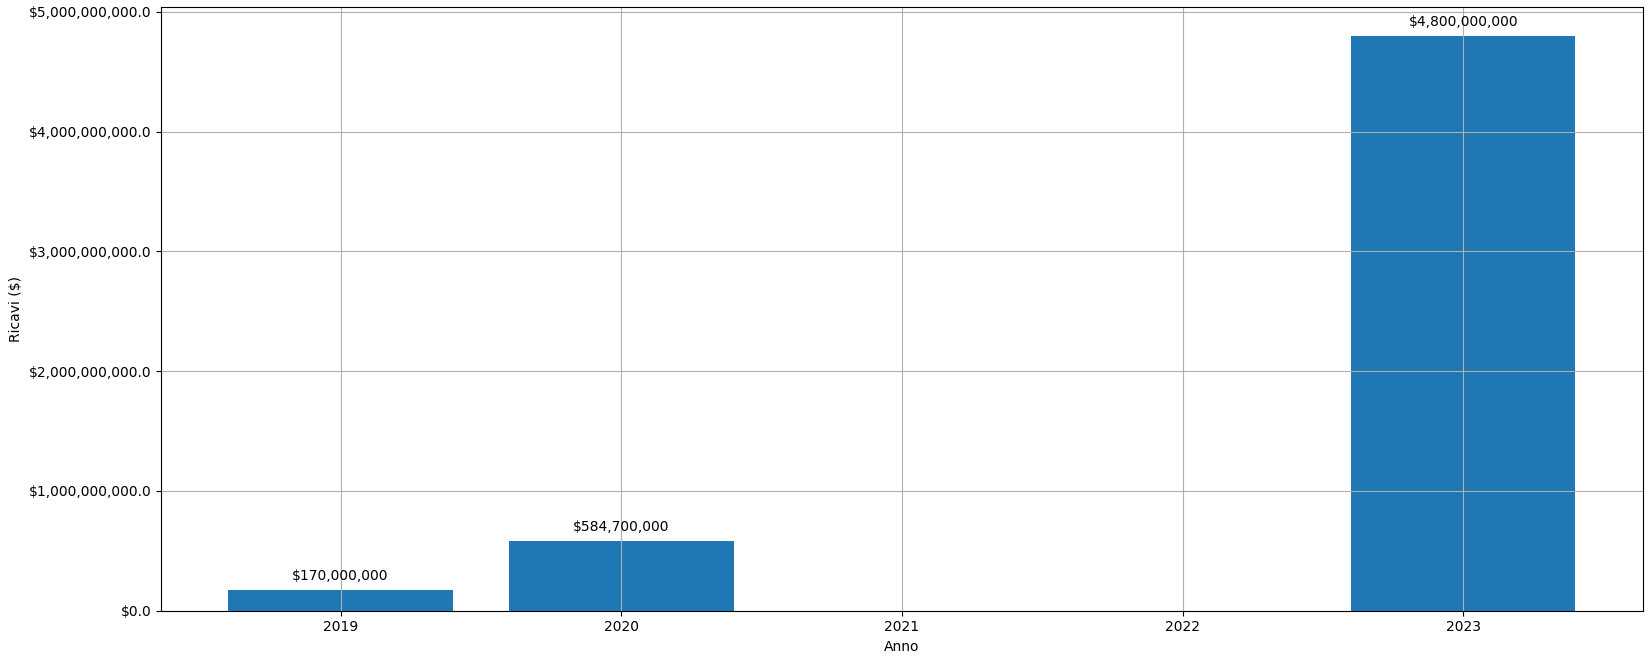
\includegraphics[width=\linewidth]{immagini/Newzoo_Cloud_Gaming_Revenues}
	\caption{Previsioni per il mercato globale del cloud gaming (in dollari americani). Fonte: newzoo.com/global-cloud-gaming-report}
	\label{fig:Newzoo_Cloud_Gaming_Revenues}
\end{figure}